\documentclass[11pt,a4paper]{article}

\usepackage[margin=1in]{geometry}
\usepackage{amsmath,amssymb,amsthm}
\usepackage{booktabs}
\usepackage{graphicx}
\usepackage{hyperref}
\usepackage{natbib}
\usepackage{xcolor}
\usepackage{setspace}
\usepackage{caption}
\usepackage{subcaption}
\usepackage{fontspec}
\usepackage[english]{babel}
\babelprovide[import,onchar=ids fonts]{chinese}

% Latin body + CM math; CJK via babel onchar (Noto Serif/Sans Mono CJK SC in TTC)
\babelfont{rm}{Latin Modern Roman}
\babelfont{tt}{Latin Modern Mono}
\babelfont[chinese]{rm}[
  Path=/usr/share/fonts/opentype/noto/,
  Extension=.ttc,
  UprightFont=NotoSerifCJK-Regular,
  BoldFont=NotoSerifCJK-Bold,
  ItalicFont=NotoSerifCJK-Regular,
  BoldItalicFont=NotoSerifCJK-Bold,
  UprightFeatures={FontIndex=2},
  BoldFeatures={FontIndex=2},
  ItalicFeatures={FontIndex=2},
  BoldItalicFeatures={FontIndex=2},
]{NotoSerifCJK}
\babelfont[chinese]{tt}[
  Path=/usr/share/fonts/opentype/noto/,
  Extension=.ttc,
  UprightFont=NotoSansCJK-Regular,
  BoldFont=NotoSansCJK-Bold,
  ItalicFont=NotoSansCJK-Regular,
  BoldItalicFont=NotoSansCJK-Bold,
  UprightFeatures={FontIndex=7},
  BoldFeatures={FontIndex=7},
  ItalicFeatures={FontIndex=7},
  BoldItalicFeatures={FontIndex=7},
  Scale=0.9,
]{NotoSansMonoCJK}

\hypersetup{
  colorlinks=true,
  linkcolor=blue!50!black,
  citecolor=blue!50!black,
  urlcolor=blue!60!black
}

\newtheorem{definition}{定义}
\newtheorem{proposition}{命题}
\newtheorem{remark}{注}

\title{通过动作聚合后的 Fisher 信息损失\\比较多智能体协调规则}
\author{
  Heath Li\\
  \texttt{Kunyanli230/Jevometry}\\
  \small 面向 JAAMAS / arXiv 的工作稿\\
  \small 本文为 \texttt{main.tex} 的中文对应译本
}
\date{\today}

\begin{document}
\maketitle

\begin{abstract}
多智能体决策系统常常把\emph{感知}——输出局部结果上范畴分布的专用智能体——与\emph{协调}——把联合结果映射到小动作字母表（例如拒绝、自动应用、升级给人工）的确定性规则——分开。尽管感知模型与联合构造在 Dec-POMDP 主动感知与信息采集中已有仔细处理，协调层却经常由启发式设计，并仅通过任务奖励或吞吐量评估。本文提出一个互补问题：\emph{在智能体输出分布固定的前提下，哪些协调规则对底层参数销毁的 Fisher 信息最少？}

我们将协调形式化为与 $\theta$ 无关的聚合映射 $A=f(Z)$，并用声明联合与其推前之间的 Fisher 信息数据处理间隙 $I_Z(\theta)-I_A(\theta)\succeq 0$ 量化信息损失。在 Jevometry 三智能体数据清洗委员会（适用性、修复、风险）及声明乘积联合下实例化该框架，我们在证据与歧义网格上比较七条纯规则——baseline、stricter、wider、quarantine-to-review、混合 quarantine-wider 拆分、粗粒度二元规则，以及近恒等上界。在设计中心点，baseline 协调约丢弃 $\mathrm{tr}(I_Z)$ 的一半；将 quarantine 软化为人工复核可挽回该损失的相当一部分；再与不同的 auto-normalize/auto-impute 标签组合，可在完整设计网格上进一步改进。粗化为二元 reject/proceed 闸门则损失更多。排序
$\mathrm{near\text{-}identity}\le\mathrm{wider}\le\mathrm{baseline}
\le\mathrm{stricter}$
在每个网格单元上稳定；$\Delta_f$ 的参数轴分解表明 quarantine 软化主要保留歧义方向。我们讨论智能体委员会的设计含义、迫使确定性映射的 API 约束，以及解析 softmax 族相对在线决策模型 API 的局限。配套代码与可复现表格随 Jevometry 仓库一并提供。
\end{abstract}

\section{引言}

大语言模型与专用决策 API 使获取看起来已校准的局部判断范畴分布变得便宜：某修复是否适用、尝试何种修复、自动写入有多危险。在生产数据系统中，这些局部判断很少是最终产物。协调器——往往是一小段确定性业务逻辑——把智能体输出的联合压缩为可执行、可延期或可拒绝的最终动作~\citep{jevometry2026}。

这种压缩是信息瓶颈。经典决策理论与 Dec-POMDP 规划优化定义在信念或预测质量上的奖励~\citep{lauri2020prediction,lauri2020decpomdp,oliehoek2016decpomdp}。信息论多智能体感知最大化互信息或相关集函数，常带有子模贪婪保证~\citep{krause2008near,nemhauser1978analysis,corah2021scalable,shi2026imas2}。这些工作选择\emph{观察什么}或\emph{谁应观察}。它们本身并不能告诉实践者：两条已部署的协调规则中，哪一条对智能体设计所跟踪的参数保留更多敏感性。

Fisher 信息为这种敏感性提供了局部、可微的语言~\citep{fisher1925theory,amari2016information}。对具有得分 Jacobian $J_Z$ 的离散模型 $P_\theta(Z)$，Fisher 矩阵 $I_Z=J_Z^\top \mathrm{diag}(P_\theta)^{-1} J_Z$ 度量无穷小参数移动如何强烈改变结果分布。当固定映射 $f$ 产生动作 $A=f(Z)$ 时，Fisher 信息的数据处理不等式在标准正则条件下断言 $I_Z-I_A\succeq 0$~\citep{zamir1998fisherdpi,cover2006elements}。当 $I_Z$ 固定时，标量 $\mathrm{tr}(I_Z-I_A)$ 便是可比较的损失摘要。

\paragraph{贡献。}
\begin{enumerate}
  \item 我们将多智能体协调规则比较表述为：在共享声明联合下，按 Fisher 信息损失对与 $\theta$ 无关的聚合映射排序（第~\ref{sec:problem}~节）。
  \item 我们在 Jevometry 清洗委员会中实例化七条纯规则，并提供可复现实验装置：扫描参数网格、导出 CSV/JSON（含参数轴损失对角元与分数损失），并生成发表用图（第~\ref{sec:method}~节）。
  \item 经验上，在设计中心点 baseline 规则约损失 $\mathrm{tr}(I_Z)$ 的 $44\%$；quarantine-to-review 相对 baseline 约削减四分之一损失；混合 quarantine-wider 规则进一步改进（$\mathrm{tr}(\Delta)\approx 2.16$）并在完整网格上优于 quarantine-to-review；二元闸门的损失高于更严的中风险拒绝（第~\ref{sec:experiments}~节）。
  \item 我们讨论该度量如何补充以奖励为中心的 Dec-POMDP 评估，以及 API 约束（仅确定性映射）对未来可学习协调器的含义（第~\ref{sec:discussion}~节）。
\end{enumerate}

本稿旨在作为伴随开源实验的短期刊 / arXiv 草稿。它并非关于在线清洗质量的主张；智能体族是解析且示意性的。

\section{相关工作}
\label{sec:related}

\paragraph{Dec-POMDP 主动感知。}
\citet{lauri2020prediction} 通过个体预测动作，将带预测奖励的多智能体主动感知约化为标准 Dec-POMDP 求解器，并给出去中心化损失界。\citet{lauri2020decpomdp} 在离散与连续状态设定下，用策略图改进优化凸信念依赖奖励（例如负熵）。两条线通常把团队视为固定，并把信息目标折入奖励，而非事后比较确定性协调器。

\paragraph{信息驱动的多智能体感知。}
子模传感器选择与多机器人跟踪在单调性下以贪婪 $(1-1/e)$ 保证最大化互信息或相关覆盖目标~\citep{krause2008near,corah2021scalable}。\citet{shi2026imas2} 在 Dec-POMDP 中为互信息目标联合选择智能体并综合感知策略。\citet{olkin2024vulcan} 与 \citet{molloy2023smoother} 进一步将规划连接到信息与平滑器熵。我们的设定是对偶的：智能体及其局部律\emph{固定}；仅最后一英里到动作的映射变化。

\paragraph{面向智能体的信息几何。}
Fisher--Rao 几何为参数化分布族提供局部度量~\citep{amari2016information}。Jevometry 为智能体系统操作化节点级与系统级 Fisher 诊断~\citep{jevometry2026}。我们使用其推前 \texttt{information\_loss} 原语，且不修改底层 DECLARED\_PRODUCT 构造。

\section{问题形式化}
\label{sec:problem}

\subsection{声明乘积联合}

令 $\theta\in\Theta\subset\mathbb{R}^d$ 参数化多智能体系统。每个智能体 $i\in\{1,\ldots,m\}$ 在有限局部字母表 $\mathcal{Z}_i$ 上发出范畴分布 $P_\theta(Z_i)$。\emph{声明乘积联合}断言给定 $\theta$ 时的条件独立：
\begin{equation}
  P_\theta(Z=z)=\prod_{i=1}^{m} P_\theta(Z_i=z_i),
  \qquad z=(z_1,\ldots,z_m)\in\mathcal{Z}=\prod_i\mathcal{Z}_i.
\end{equation}
在我们的清洗例子中，$m=3$，$d=2$，且 $\theta=(\mathrm{evidence},\mathrm{ambiguity})$，坐标在 $[0,1]$。该声明是模型假设，而非关于在线 API 的经验主张。

\subsection{作为聚合的协调}

\begin{definition}[协调规则]
协调规则是映射 $f:\mathcal{Z}\to\mathcal{A}$，映入有限动作字母表 $\mathcal{A}$。若 $f$ 仅是联合结果的全函数（无隐随机性），则称其为\emph{纯}的；若 $f$ 不依赖 $\theta$，则称其为\emph{与 $\theta$ 无关}的。
\end{definition}

诱导的动作律是推前
\begin{equation}
  P_\theta(A=a)=\sum_{z:f(z)=a} P_\theta(Z=z).
\end{equation}
若 $J_Z(\theta)$ 是联合概率向量关于 $\theta$ 的 Jacobian，则聚合 Jacobian $J_A$ 通过对共享同一动作标签的 $J_Z$ 行求和得到。

\subsection{Fisher 信息损失}

\begin{definition}[规则的信息损失]
对与 $\theta$ 无关的规则 $f$，定义
\begin{align}
  I_Z(\theta) &= J_Z(\theta)^\top \mathrm{diag}\bigl(P_\theta(Z)\bigr)^{-1} J_Z(\theta),\\
  I_A(\theta) &= J_A(\theta)^\top \mathrm{diag}\bigl(P_\theta(A)\bigr)^{-1} J_A(\theta),\\
  \Delta_f(\theta) &= I_Z(\theta)-I_A(\theta).
\end{align}
我们报告 $\mathrm{tr}(I_Z)$、$\mathrm{tr}(I_A)$ 与 $\mathrm{tr}(\Delta_f)$ 作为标量摘要，并数值验证 $\Delta_f\succeq 0$（PSD 检查）作为数据处理诊断。
\end{definition}

\begin{proposition}[固定映射的 DPI]
在标准正性与可微条件下，任意与 $\theta$ 无关的 $f$ 满足 $\Delta_f(\theta)\succeq 0$。当 $f$ 在 $P_\theta$ 的支撑上单射时等号成立。
\end{proposition}

\begin{remark}
依赖 $\theta$ 的映射（软策略、以参数为条件的学习路由）落在 Jevometry 实现的该保证之外，并被报告为不支持。因此本文仅关注纯的、全覆盖的、与 $\theta$ 无关的规则——即匹配典型生产 if-then 协调器与库的 AggregationMap 契约的那一类。
\end{remark}

\paragraph{比较原则。}
固定智能体与联合构造。按 $\mathrm{tr}(\Delta_f)$ 对规则排序（越低越好），或等价地按 $\mathrm{tr}(I_A)$（越高越好）。因为 $I_Z$ 共享，按损失排序与按保留信息排序相同。

\section{方法与实验设计}
\label{sec:method}

\subsection{三智能体清洗委员会}

我们复用离线 Jevometry 教程 \texttt{examples/three\_agent\_cleaning}~\citep{jevometry2026}。三个解析 softmax 智能体为噪声数值字段的单个候选修复产生分布：

\begin{center}
\begin{tabular}{lll}
\toprule
智能体 & 原语 & 支撑 \\
\midrule
applicability & Noul & $\{\mathrm{false},\mathrm{true}\}$ \\
repair & Choice & $\{\mathrm{normalize},\mathrm{impute},\mathrm{quarantine}\}$ \\
risk & Score & $\{0,1,2\}$（低/中/高） \\
\bottomrule
\end{tabular}
\end{center}

局部 logit 在设计中心 $\theta_0=(0.7,0.3)$ 附近对 $(\theta-\theta_0)$ 为仿射，概率由 softmax 得到。联合是声明乘积（ConstructionMode.DECLARED\_PRODUCT）。不查询任何在线 API；不执行实际数据库写入。

\subsection{协调规则}
\label{sec:rules}

我们比较七条规则，均为纯且与 $\theta$ 无关：

\begin{description}
  \item[baseline] 若不适用、quarantine 或高风险则拒绝；若 normalize 且低风险则自动应用；否则人工复核。
  \item[stricter] 同 baseline，但中风险也拒绝。
  \item[wider] 拒绝条件同 baseline；低风险 normalize 与 impute 成为不同的自动标签（\texttt{auto\_normalize}、\texttt{auto\_impute}）。
  \item[quarantine\_review] Quarantine 路由到人工复核而非拒绝；仅在不适用或高风险时拒绝。
  \item[quarantine\_wider] Quarantine-to-review 与 wider 的双自动标签组合：本研究中经验上最强的粗策略。
  \item[coarse\_binary] 在 baseline 拒绝条件下拒绝；否则为单一 \texttt{proceed} 动作（自动应用与复核合并）。
  \item[near\_identity] 每个联合结果元组一个动作标签（18 个标签）：在该字母表下的 Fisher 保留上界。
\end{description}

\subsection{实验装置}

脚本 \texttt{paper\_experiments.py} 一次构建节点与联合，在 $\mathrm{evidence}\in[0.2,0.9]$ 与 $\mathrm{ambiguity}\in[0.1,0.8]$ 的 $8\times 8$ 网格上评估 $I_Z$、$I_A$ 与 $\Delta_f$，并额外记录精确中心 $\theta_0$。输出：

\begin{itemize}
  \item \texttt{papers/coord-fisher/data/rule\_loss\_grid.\{csv,json\}}
  \item \texttt{papers/coord-fisher/data/center\_summary.json}
  \item \texttt{papers/coord-fisher/data/center\_loss\_anisotropy.csv}、
  \texttt{rule\_loss\_anisotropy\_grid.csv}、分数损失热图
  \item \texttt{papers/coord-fisher/data/iteration\_summary.json}
  \item 图~\ref{fig:center}--\ref{fig:masses}，位于
  \texttt{papers/coord-fisher/figures/}
\end{itemize}

\texttt{src/jevometry} 下的库代码未改动；仅扩展了示例级规则与脚本。

\section{实验}
\label{sec:experiments}

\subsection{中心点排序}

表~\ref{tab:center} 报告 $\theta_0$ 处的迹。所有规则返回状态 \texttt{ok}，损失矩阵为 PSD。近恒等映射无损失（至多数值噪声），对照 DPI 等号情形确认实现。Baseline 损失 $\mathrm{tr}(\Delta)\approx 3.03$，出自 $\mathrm{tr}(I_Z)\approx 6.84$——约 $44\%$。Wider 通过保留不同自动路径而略优于 baseline。更严的中风险拒绝增加损失。将 quarantine 软化为复核带来显著实际收益（$\mathrm{tr}(\Delta)\approx 2.27$）；将该软化与 wider 的双自动标签叠加以得到 \texttt{quarantine\_wider}，进一步改进至 $\approx 2.16$，是此处最佳的非恒等粗策略。坍缩为二元闸门在所列规则中最差（$\approx 3.71$）。

\begin{table}[t]
\centering
\caption{中心 $\theta_0=(0.7,0.3)$ 处的 Fisher 迹，按损失升序排列。
$|A|$ 为推前下具有正质量的动作数。}
\label{tab:center}
\begin{tabular}{lrrrrl}
\toprule
规则 & $\mathrm{tr}(I_Z)$ & $\mathrm{tr}(I_A)$ & $\mathrm{tr}(\Delta)$ & $|A|$ & 状态 \\
\midrule
near\_identity & 6.8418 & 6.8418 & 0.0000 & 18 & ok \\
quarantine\_wider & 6.8418 & 4.6816 & 2.1602 & 4 & ok \\
quarantine\_review & 6.8418 & 4.5764 & 2.2654 & 3 & ok \\
wider & 6.8418 & 3.8285 & 3.0133 & 4 & ok \\
baseline & 6.8418 & 3.8080 & 3.0338 & 3 & ok \\
stricter & 6.8418 & 3.4198 & 3.4220 & 3 & ok \\
coarse\_binary & 6.8418 & 3.1296 & 3.7122 & 2 & ok \\
\bottomrule
\end{tabular}
\end{table}

先前探索工作中强调的核心排序在 $8\times 8$ 设计网格的\emph{每一个}单元上（$64/64$）仍然成立，而不仅在中心（数值容差 $10^{-9}$）：
\begin{equation*}
  \mathrm{near\text{-}identity}
  \;\le\;
  \mathrm{wider}
  \;\le\;
  \mathrm{baseline}
  \;\le\;
  \mathrm{stricter}
\end{equation*}
Quarantine-to-review 在损失轴上插在 wider \emph{之下}；\texttt{quarantine\_wider} 插得更低，并在 $65/65$ 次记录的中心与网格评估上满足
$\mathrm{tr}(\Delta_{\mathrm{quarantine\_wider}})
\le\mathrm{tr}(\Delta_{\mathrm{quarantine\_review}})$。
粗二元规则位于 stricter \emph{之上}——相对原先四规则故事的有信息偏离。

\begin{figure}[t]
\centering
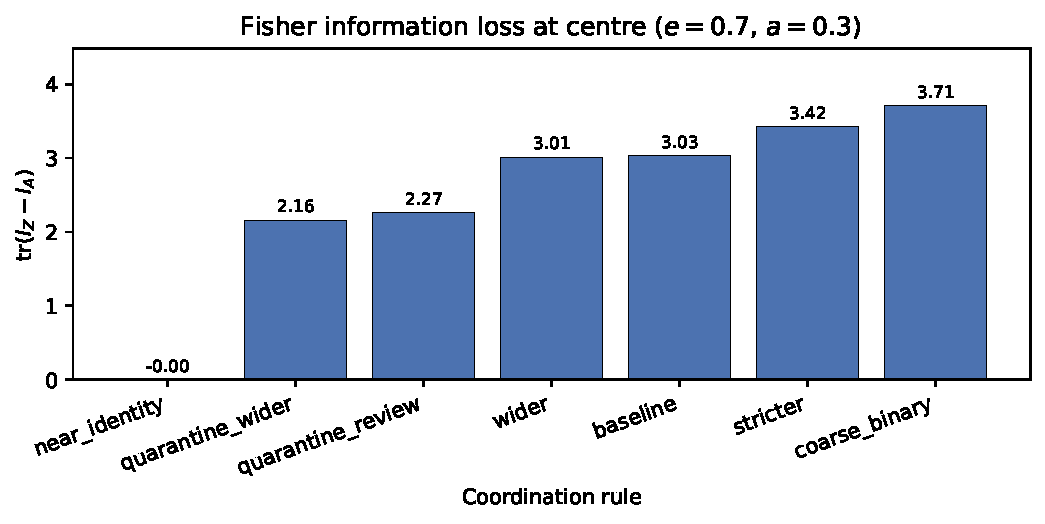
\includegraphics[width=0.85\linewidth]{figures/fig_loss_center.pdf}
\caption{设计中心处各规则的信息损失 $\mathrm{tr}(I_Z-I_A)$。}
\label{fig:center}
\end{figure}

\subsection{网格行为}

图~\ref{fig:heat} 给出五条非恒等规则在参数网格上的损失热图。绝对损失随 $\theta$ 变化，因为 $I_Z(\theta)$ 与跨 $f$-纤维的质量分配都在变，但定性排序在定义域的大片区域稳定：更软、更细的动作字母表比更严或二元闸门更“冷”（损失更低）。图~\ref{fig:curves} 在歧义最接近 $0.3$ 处切片损失对证据的关系；近恒等保持为零，而粗二元与 stricter 仍是损失最大的。

\begin{figure}[t]
\centering
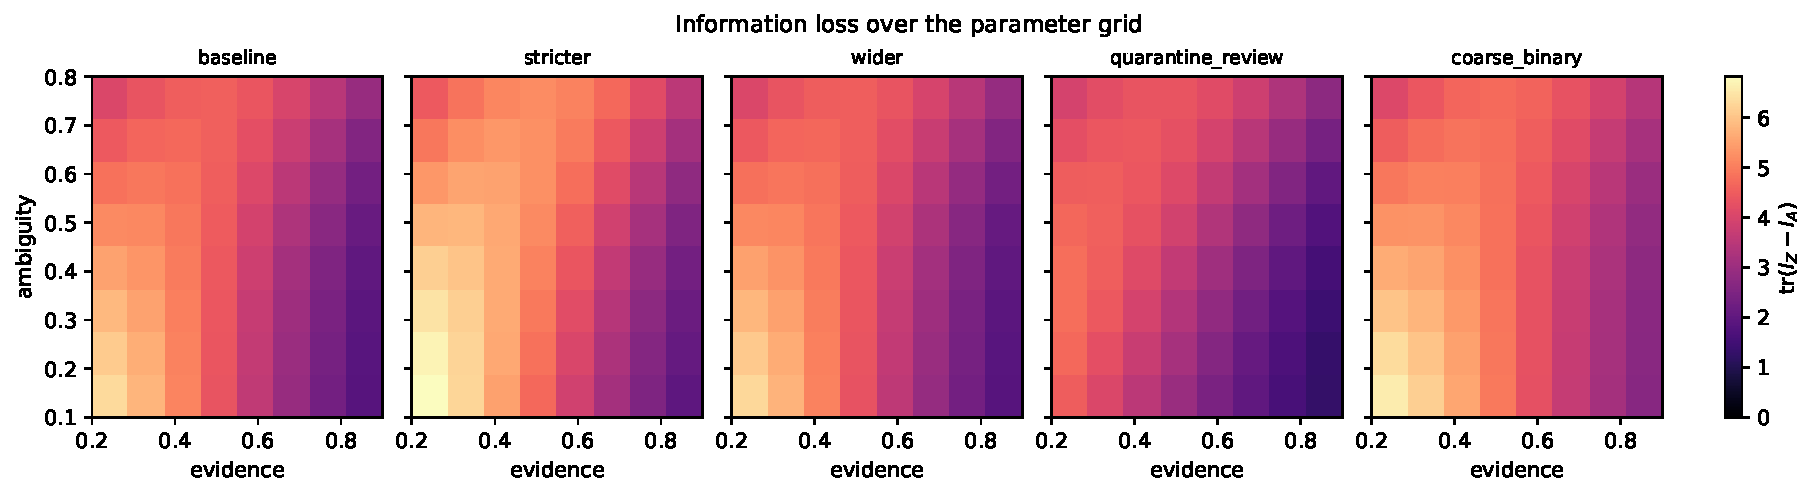
\includegraphics[width=\linewidth]{figures/fig_loss_heatmap.pdf}
\caption{五条协调规则在 evidence$\times$ambiguity 上的损失热图。}
\label{fig:heat}
\end{figure}

\begin{figure}[t]
\centering
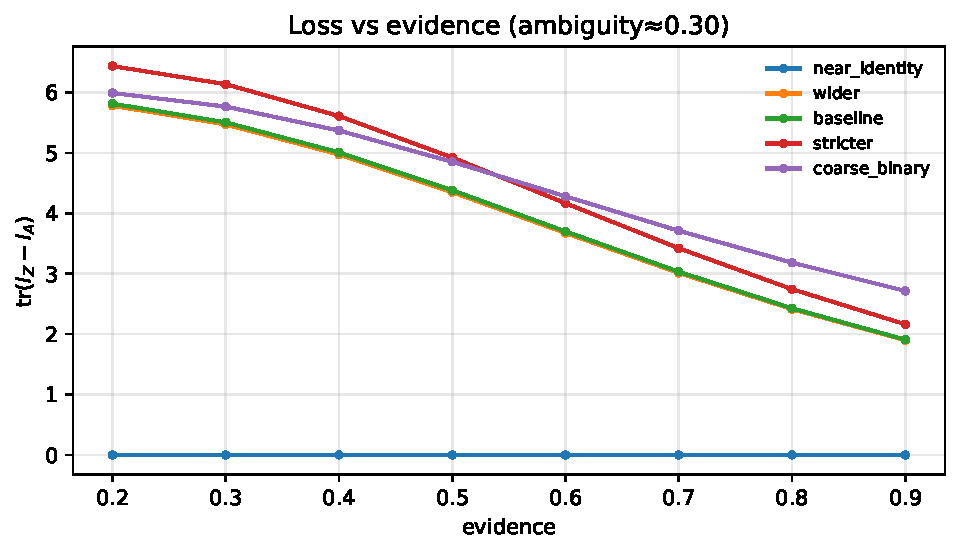
\includegraphics[width=0.85\linewidth]{figures/fig_loss_curves.pdf}
\caption{在固定歧义约 $0.3$ 处损失相对证据的变化。}
\label{fig:curves}
\end{figure}

\subsection{动作质量}

图~\ref{fig:masses} 显示中心处概率质量如何划分。Stricter 把中风险质量再分配到拒绝。Wider 把自动应用拆成 normalize 与 impute。Quarantine-to-review 缩小拒绝、偏向人工复核。粗二元把自动应用与复核折叠进 \texttt{proceed}。这些质量转移正是 Fisher 损失背后的机制：合并得分行相异的结果会坍缩可区分的参数方向。

\begin{figure}[t]
\centering
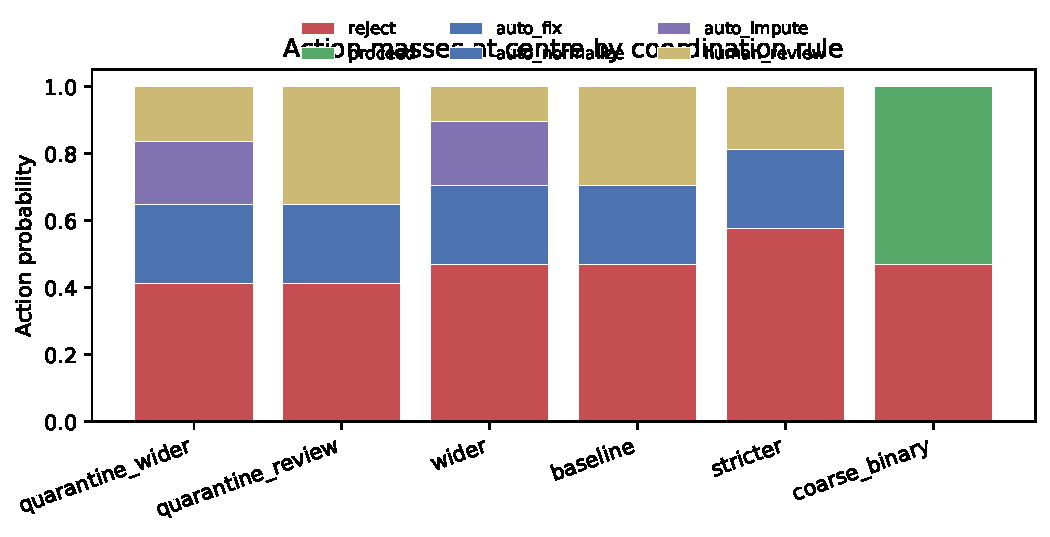
\includegraphics[width=0.85\linewidth]{figures/fig_action_masses.pdf}
\caption{非恒等规则在中心处的推前动作概率。}
\label{fig:masses}
\end{figure}

\subsection{各向异性与 quarantine-wider 机制}
\label{sec:anisotropy}

迹摘要掩盖了哪一参数方向被丢弃。在 $\theta_0$，$(\mathrm{evidence},\mathrm{ambiguity})$ 基下 $\Delta_f$ 的对角元表明：相对 baseline，\texttt{quarantine\_review} 大约将歧义轴损失减半（$\Delta_{aa}\approx 0.95$ 对 $\approx 1.69$），而证据轴损失保持可比。相对损失 $\mathrm{tr}(\Delta)/\mathrm{tr}(I_Z)$ 在网格上 $I_Z(\theta)$ 变化处保持相同排序。

推前质量解释混合收益：相对 \texttt{quarantine\_review}，\texttt{quarantine\_wider} 用不同的 \texttt{auto\_normalize} 与 \texttt{auto\_impute} 原子替换单一 \texttt{auto\_apply} 原子，并把额外质量从 \texttt{human\_review} 移入 \texttt{auto\_impute}；\texttt{reject} 质量不变。更细的自动纤维保留了较粗复核规则所合并的得分行。

\begin{figure}[t]
\centering
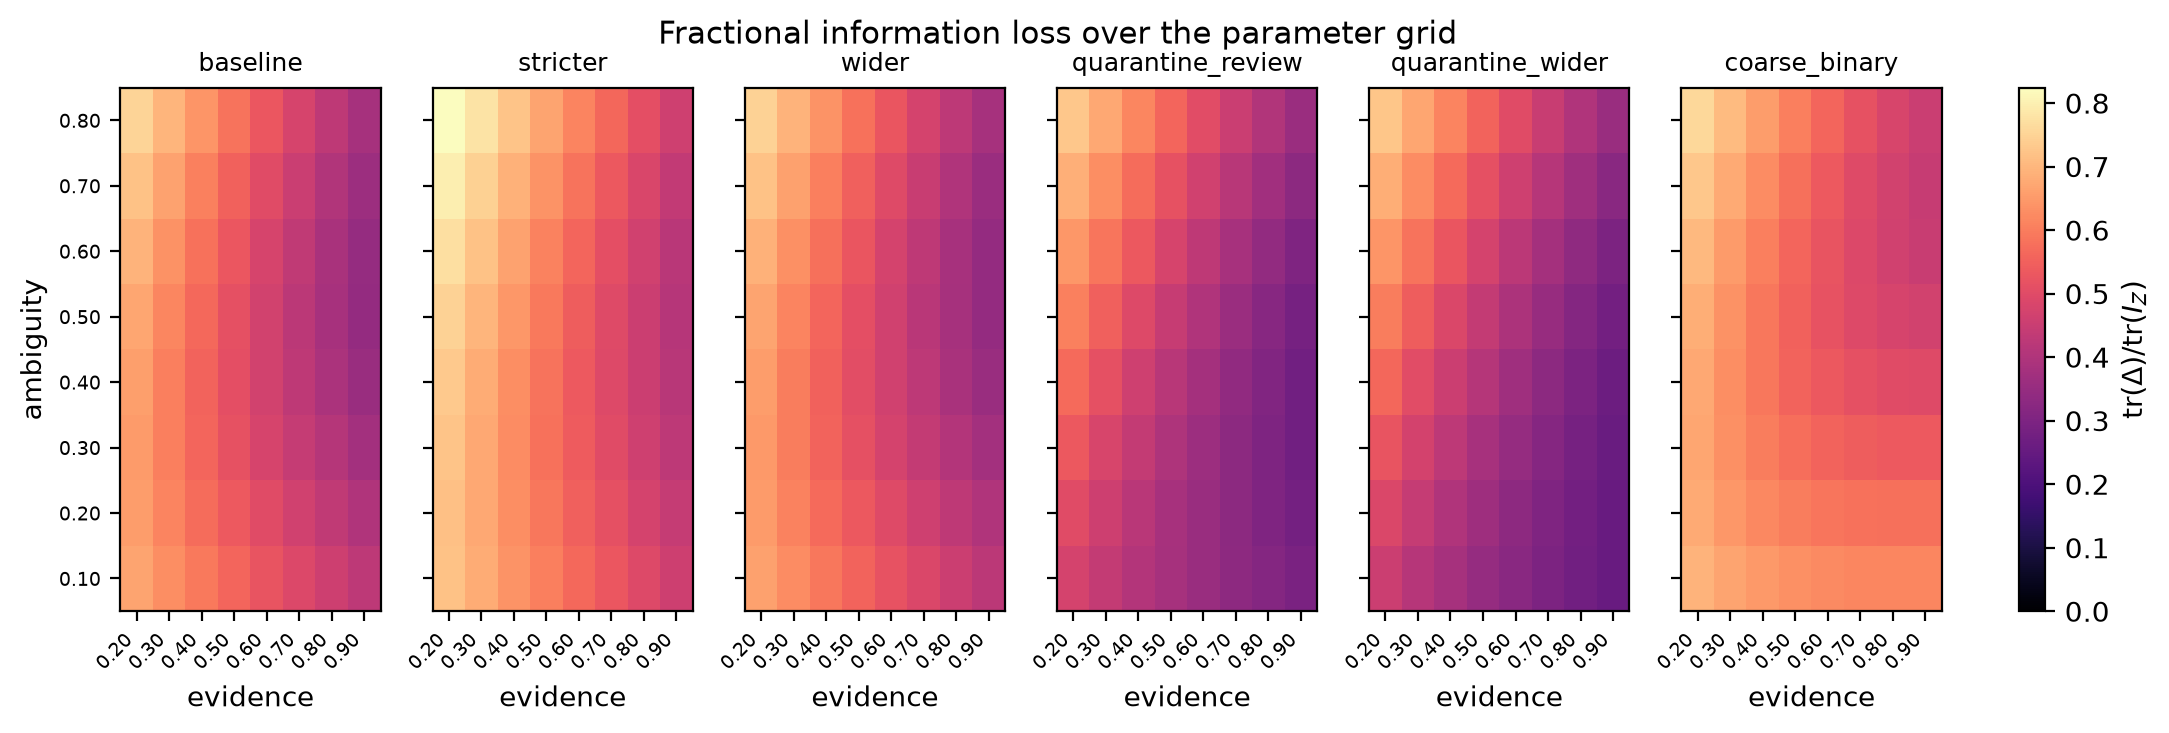
\includegraphics[width=0.9\linewidth]{figures/fig_frac_loss_heatmap.png}
\caption{非恒等规则在 evidence$\times$ambiguity 网格上的分数损失 $\mathrm{tr}(\Delta)/\mathrm{tr}(I_Z)$。}
\label{fig:frac}
\end{figure}

\section{讨论}
\label{sec:discussion}

\paragraph{“一半 Fisher”意味着什么。}
Baseline 协调后 $\mathrm{tr}(I_Z)$ 下降 $44\%$ 并不意味着系统“错了” $44\%$。它意味着：局部上，证据与歧义的无穷小变化对最终动作分布的推动，弱于对智能体输出联合的推动。若监控仪表盘只看动作率，就会低估底层委员会的敏感性。若下游估计器试图从动作反推 $\theta$，其问题严格难于从 $Z$ 反推。

\paragraph{设计要点。}
在可实现的三/四动作策略中，将 quarantine 路由到复核比单独的 baseline 或 wider 保留更多 Fisher；将该软化与不同的 auto-normalize/auto-impute 标签组合，在本网格上仍严格更好。二元 proceed/reject 闸门在运维上方便，但在信息上昂贵。实践者在 A/B 测试前讨论规则变更时，可将 $\mathrm{tr}(\Delta_f)$——以及需要时其参数轴对角元——当作廉价的离线评分。

\paragraph{与 Dec-POMDP 奖励的关系。}
预测奖励与负熵目标~\citep{lauri2020prediction,lauri2020decpomdp} 优化感知策略。我们的度量并不取代它们；它在感知固定之后审计\emph{最后}一道确定性压缩。就此意义而言，它与 IMAS$^2$ 风格的联合选择~\citep{shi2026imas2} 互补：选择扩展谁可以观察；协调排序追问这些观察有多少在动作层幸存。

\paragraph{API 约束。}
许多智能体平台仅暴露采样结果加确定性业务规则。软的、依赖 $\theta$ 的路由器要么需要声明条件动作模型，要么拒绝 DPI 证书——正是 Jevometry AggregationMap 所编码的契约。将本研究扩展到随机协调器是未来工作，并需要额外正则性。

\section{局限}
\label{sec:limitations}

\begin{itemize}
  \item 智能体分布是手工指定的解析 softmax 族，而非拟合的在线决策模型。绝对数值是示意性的。
  \item 条件独立是声明的，而非检验的。
  \item 我们报告 $\Delta_f$ 的参数轴对角元与特征值，但完整 CRLB 式解读仍需要本例未提供的观测似然契约。
  \item 各规则的动作字母表不同；作为关于 $\theta$ 的保留信息，$\mathrm{tr}(I_A)$ 比较仍然有意义，但把 $|A|$ 当作效用的解释超出范围。
  \item 没有人工或任务奖励研究验证更低的 Fisher 损失会改善清洗结果。
\end{itemize}

\section{结论}
\label{sec:conclusion}

我们提出在共享声明联合下按 Fisher 信息损失对多智能体协调规则排序，并在可复现的三智能体清洗委员会上展示该方法。在感知固定时，确定性协调器可丢弃联合 Fisher 迹量级约一半；小的规则编辑（quarantine 处理、自动路径拆分、风险阈值）及其组合会以易于离线度量的幅度——包括沿各参数轴——移动该损失。配套实验装置与图旨在作为在变更在线流量前审计生产 if-then 委员会的模板。

未来工作包括：(i) 在同一 AggregationMap 接口下用 TypeSafe / 在线决策模型 Jacobian 替换解析智能体；(ii) 带显式条件动作模型的随机协调器；(iii) 在 JAAMAS 风格的经验研究中将 $\mathrm{tr}(\Delta_f)$ 与任务级效用耦合。

\section*{可复现性}

从仓库根目录：
\begin{verbatim}
uv sync --locked
uv pip install matplotlib   # paper figures
uv run python examples/three_agent_cleaning/compare_rules.py
uv run python examples/three_agent_cleaning/paper_experiments.py
\end{verbatim}
产物落在 \texttt{papers/coord-fisher/data} 与
\texttt{figures/}。本 PDF 由 lualatex 自
\texttt{papers/coord-fisher/main-zh.tex} 构建（英文版见 \texttt{main.tex}）。

\bibliographystyle{plainnat}
\bibliography{references}

\end{document}
